\section{Diseño matemático}
\label{sec:diseno}

\subsection{Aproximaciones utilizadas}

\subsubsection{Chebyshev~I}
La aproximación de Chebyshev~I distribuye el error en forma equirrizada en la banda de paso y es monótona en la banda de rechazo.
Sobre el prototipo pasabajos normalizado ($\Omega = \omega/\omega_p$):
\begin{equation}
  \lvert H(j\Omega)\rvert^2 = \frac{1}{1+\varepsilon^2 C_N^2(\Omega)}, \qquad
  C_N(\Omega) =
  \begin{cases}
    \cos\!\left(N\arccos\Omega\right), & \lvert\Omega\rvert \le 1,\\
    \cosh\!\left(N\,\mathrm{arccosh}\,\Omega\right), & \lvert\Omega\rvert > 1,
  \end{cases}
  \label{eq:cheby}
\end{equation}
con $\varepsilon^2 = 10^{A_p/10}-1$ ($\varepsilon = \num{0.5088}$ para $A_p = \qty{1}{\decibel}$). Exigir $A(\Omega_s) \ge A_s$ conduce al orden mínimo
\begin{equation}
  N \ge \frac{\mathrm{arccosh}\sqrt{D}}{\mathrm{arccosh}\,\Omega_s}, \qquad D = \frac{10^{A_s/10}-1}{10^{A_p/10}-1},
  \label{eq:orden_cheby}
\end{equation}
con $\sqrt{D} = \num{31.085}$. Los polos se ubican sobre una elipse:
\begin{equation}
  \begin{gathered}
  p_k = \omega_p\left[-\sinh a\,\sin\theta_k + j\cosh a\,\cos\theta_k\right],\qquad k = 1,\dots,N,\\
  a = \frac{1}{N}\,\mathrm{arcsinh}\frac{1}{\varepsilon},\qquad \theta_k = \frac{(2k-1)\pi}{2N}.
  \end{gathered}
  \label{eq:polos_cheby}
\end{equation}
Como $C_N(0) = 0$ para $N$ impar y $\lvert C_N(0)\rvert = 1$ para $N$ par, la ganancia en continua es \qty{0}{\decibel} en el primer caso y $-A_p$ en el segundo.

\subsubsection{Elíptica (Cauer)}
La aproximación elíptica es equirrizada en ambas bandas:
\begin{equation}
  \lvert H(j\Omega)\rvert^2 = \frac{1}{1+\varepsilon^2 R_N^2(\Omega)},
  \label{eq:elip}
\end{equation}
donde $R_N$ es la función racional de Chebyshev (o elíptica), que oscila entre $\pm1$ para $\lvert\Omega\rvert\le1$ y cumple
$\lvert R_N\rvert \ge \sqrt{D}$ para $\lvert\Omega\rvert \ge \Omega_s$. Sus polos sobre el eje imaginario son \emph{ceros de transmisión}
de $H$, lo que produce la transición más abrupta posible para un orden dado. El orden mínimo surge de la ecuación de grado
\begin{equation}
  N \ge \frac{K(k)\,K\!\left(\sqrt{1-k_1^2}\right)}{K\!\left(\sqrt{1-k^2}\right)K(k_1)},\qquad k = \frac{1}{\Omega_s},\qquad k_1 = \frac{1}{\sqrt{D}},
  \label{eq:orden_elip}
\end{equation}
donde $K(\cdot)$ es la integral elíptica completa de primera especie. Para $N$ par, $\lvert H(0)\rvert$ vale $-A_p$ y
$\lvert H(j\infty)\rvert$ vale $-A_s$: la atenuación en alta frecuencia no crece indefinidamente.

\subsubsection{Transformación pasabajos--rechazabanda}
El rechazabanda se obtiene del prototipo pasabajos mediante
\begin{equation}
  s_{LP} = \frac{B\,s}{s^2+\omega_0^2},\qquad \omega_0^2 = \omega_{p1}\,\omega_{p2},\qquad B = \omega_{p2}-\omega_{p1},
  \label{eq:transf_bs}
\end{equation}
que en el eje $\jw$ da $\Omega(\omega) = B\omega/(\omega_0^2-\omega^2)$: los bordes de paso van a $\Omega = 1$ y cada borde de rechazo a
$\Omega(\omega_{s,i})$. El prototipo debe cumplir el peor caso, $\Omega_s = \min_i \lvert\Omega(\omega_{s,i})\rvert$. Cada polo del prototipo
genera un par de polos (el orden se duplica), los ceros en infinito del prototipo se transforman en ceros sobre $\pm j\omega_0$ y cada cero
finito $\pm j\Omega_z$ genera dos pares de ceros con simetría geométrica respecto de $\omega_0$.

\paragraph{Asimetría de la plantilla BS.} La plantilla no es geométricamente simétrica:
$500\times5500 = \qty{2.75e6}{\hertz\squared}$, mientras que $1200\times2400 = \qty{2.88e6}{\hertz\squared}$. Con los bordes de paso
especificados, el borde de rechazo de \qty{2400}{\hertz} resulta el peor caso ($\Omega_s = \num{3.987}$) y Chebyshev~I requiere
$N = \num{2.005} \to 3$, es decir, un rechazabanda de orden~6. Sin embargo, la especificación solo exige banda de paso \emph{hasta}
\qty{500}{\hertz}: ensanchar el borde inferior a
\begin{equation}
  f_{p1}' = \frac{f_{s1} f_{s2}}{f_{p2}} = \frac{1200\times2400}{5500} = \qty{523.6}{\hertz} \;\ge\; \qty{500}{\hertz}
\end{equation}
es más exigente que la plantilla (la contiene) y vuelve simétrico el problema, con $\Omega_s = \num{4.147}$ y $N = \num{1.966} \to 2$
(orden total~4). La alternativa de mover el borde superior ($f_{p2}' = 2{,}88\times10^6/500 = \qty{5760}{\hertz}$) no es válida porque
\emph{estrecharía} la banda de paso. Se ahorra así una sección bicuadrática completa sin violar ninguna especificación; es el mismo criterio
que aplican \texttt{cheb1ord} y \texttt{ellipord} para filtros de banda. La \cref{tab:orden} resume el cálculo analítico, que coincide
con SciPy en los cuatro casos.

\begin{table}[H]
  \centering\small
  \caption{Orden mínimo según las \cref{eq:orden_cheby,eq:orden_elip}. Para el BS, $N$ es el orden del prototipo (orden total $2N$).}
  \label{tab:orden}
  \tabres{tab_orden}
\end{table}

\subsection{Resultados de los cuatro diseños}

Los diseños se obtuvieron con \texttt{cheb1ord}/\texttt{ellipord} (orden y frecuencia de diseño) y \texttt{cheby1}/\texttt{ellip} con
\texttt{analog=True} y \texttt{output='zpk'}. Para Chebyshev~I y la elíptica la frecuencia de diseño es el borde de la banda de rizado:
$f_p = \qty{1000}{\hertz}$ (LP) y $f_{p1}' = \qty{523.64}{\hertz}$, $f_{p2} = \qty{5500}{\hertz}$ (BS). Todos los polos tienen parte real
negativa (diseños estables). Cada par de polos complejos $p,\bar p$ define una sección $s^2 + (\omega_0/Q)s + \omega_0^2$ con
\begin{equation}
  \omega_0 = \lvert p\rvert, \qquad Q = \frac{\lvert p\rvert}{-2\,\mathrm{Re}\,p},
  \label{eq:w0Q}
\end{equation}
y cada polo real $-\sigma$ una sección $s+\sigma$. Los ceros sobre el eje $\jw$ se aparean con el par de polos de $\omega_0$ más cercano.
La \cref{tab:secciones} resume las secciones y la \cref{fig:polos_ceros} muestra los diagramas de polos y ceros.

\begin{table}[H]
  \centering\small
  \caption{Descomposición de los cuatro diseños en secciones de primer y segundo orden.}
  \label{tab:secciones}
  \tabres{tab_secciones}
\end{table}

\begin{figure}[H]
  \centering
  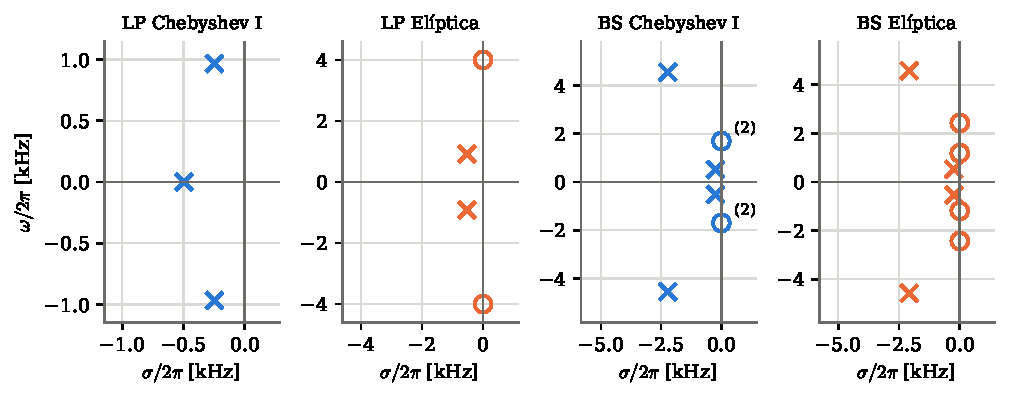
\includegraphics[width=\linewidth]{fig_polos_ceros}
  \caption{Polos ($\times$) y ceros ($\circ$) de los cuatro diseños, en el plano $s/2\pi$ [kHz]. El número entre paréntesis indica
  multiplicidad: el BS Chebyshev~I tiene ceros dobles en $\pm j\,2\pi\cdot\qty{1697.1}{\hertz}$.}
  \label{fig:polos_ceros}
\end{figure}

\paragraph{LP Chebyshev~I (orden~3).}
\begin{equation}
  H(s) = \frac{\num{1.2187e11}}{s^3 + \num{6209.9}\,s^2 + \num{4.8890e7}\,s + \num{1.2187e11}}
       = \underbrace{\frac{\omega_r}{s+\omega_r}}_{T_1(s)}\;
         \underbrace{\frac{\omega_0^2}{s^2 + \frac{\omega_0}{Q}s + \omega_0^2}}_{T_2(s)},
  \label{eq:H_LP_cheb}
\end{equation}
con $\omega_r = \qty{3105.0}{\radian\per\second}$ ($f_r = \qty{494.2}{\hertz}$), $\omega_0 = \qty{6265.0}{\radian\per\second}$
($f_0 = \qty{997.1}{\hertz}$) y $Q = \num{2.018}$; $H(0) = 1$ (\qty{0}{\decibel}). Los polos de la \cref{eq:polos_cheby} coinciden con los
de SciPy con error relativo $\num{4e-16}$. Para $N = 3$ se verifica además que $\omega_0/Q = \omega_r$, pues $\sin\theta_2 = 1$ y
$\sin\theta_1 = 1/2$ en la \cref{eq:polos_cheby}.

\paragraph{LP elíptico (orden~2).}
\begin{equation}
  H(s) = \num{0.063096}\,\frac{s^2 + \omega_z^2}{s^2 + \frac{\omega_0}{Q}s + \omega_0^2},
  \label{eq:H_LP_elip}
\end{equation}
con $\omega_z = \qty{25166}{\radian\per\second}$ ($f_z = \qty{4005.3}{\hertz}$), $\omega_0 = \qty{6696.0}{\radian\per\second}$
($f_0 = \qty{1065.7}{\hertz}$) y $Q = \num{1.009}$. Resulta $H(0) = \num{0.8913}$ (\qty{-1}{\decibel}) y $H(j\infty) = \num{0.0631}$
(\qty{-24}{\decibel}).

\paragraph{BS Chebyshev~I (orden~4).}
\begin{equation}
  H(s) = H_0 \prod_{i=1}^{2} \frac{\omega_{0i}^2}{\omega_z^2}\,\frac{s^2+\omega_z^2}{s^2 + \frac{\omega_{0i}}{Q_i}s + \omega_{0i}^2},
  \qquad H_0 = \num{0.8913},
  \label{eq:H_BS}
\end{equation}
con ceros dobles en $\omega_z = \qty{10663}{\radian\per\second}$ ($f_z = \qty{1697.1}{\hertz} = \sqrt{1200\times2400}$\,Hz) y secciones
$f_{01} = \qty{568.4}{\hertz}$, $f_{02} = \qty{5066.8}{\hertz}$, ambas con $Q = \num{1.137}$. Los dos pares de polos son geométricamente
simétricos: $\omega_{01}\omega_{02} = \omega_z^2$.

\paragraph{BS elíptico (orden~4).} Misma forma que la \cref{eq:H_BS}, pero cada sección tiene su propio cero:
$f_{z1} = \qty{1186.0}{\hertz}$ (sección $f_{01} = \qty{572.9}{\hertz}$, $Q = \num{1.210}$) y $f_{z2} = \qty{2428.4}{\hertz}$ (sección
$f_{02} = \qty{5026.9}{\hertz}$, $Q = \num{1.210}$). La primera es una sección \emph{notch} pasabajos ($f_z > f_0$) y la segunda una
\emph{notch} pasaaltos ($f_z < f_0$); $f_{z1}f_{z2} = f_{01}f_{02} = \qty{2.88e6}{\hertz\squared}$.

\subsection{Verificación de especificaciones}

La atenuación se evaluó en una grilla logarítmica densa (\num{3000} puntos por banda, incluidos los bordes exactos) sobre toda la banda de
paso (desde \qty{1}{\hertz}) y toda la banda de rechazo (hasta \qty{1}{\mega\hertz}). La \cref{tab:verificacion} muestra que los cuatro
diseños cumplen y que ninguno cumple con un orden de prototipo menor, lo que confirma que el orden es mínimo.

\begin{table}[H]
  \centering
  \caption{Verificación de la plantilla. Margen: $A_{s,\min} - A_s$.}
  \label{tab:verificacion}
  \footnotesize
  \tabres{tab_verificacion}
\end{table}

Dos observaciones. Primero, el LP Chebyshev~I de orden~3 cumple con \qty{17.9}{\decibel} de margen a \qty{4}{\kilo\hertz}, porque el orden~2
falla por muy poco ($N = \num{2.001}$ en la \cref{tab:orden}) y el salto a orden~3 sobredimensiona la selectividad. Segundo, los diseños
elípticos tienen margen nulo en la banda de rechazo por construcción: SciPy fija el rizado de rechazo exactamente en $A_s$ y aprovecha
el orden sobrante para adelantar la transición (el LP elíptico alcanza \qty{24}{\decibel} a \qty{2877}{\hertz}, no a \qty{4000}{\hertz}).
La frecuencia de \qty{-3}{\decibel} es \qty{1094.9}{\hertz} para el Chebyshev~I y \qty{1199.7}{\hertz} para el elíptico.

\subsection{Comparación}

\subsubsection{Magnitud}

\begin{figure}[H]
  \centering
  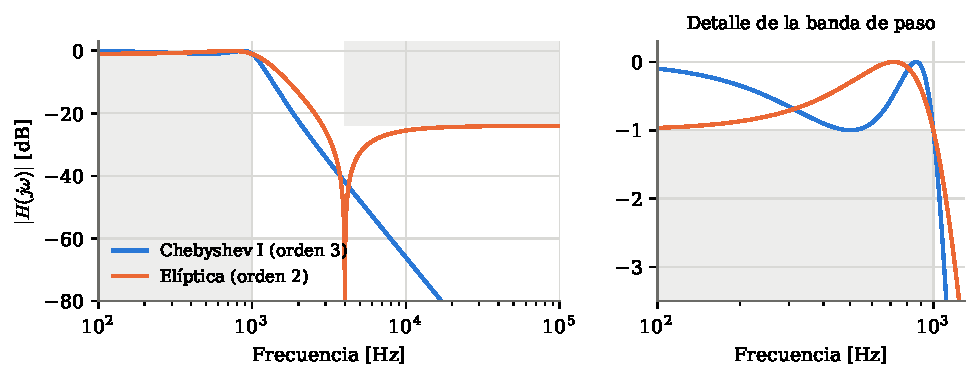
\includegraphics[width=\linewidth]{fig_LP_magnitud}
  \caption{Pasabajos: magnitud de ambas aproximaciones. Las zonas grises son las regiones prohibidas de la plantilla.}
  \label{fig:LP_mag}
\end{figure}

\begin{figure}[H]
  \centering
  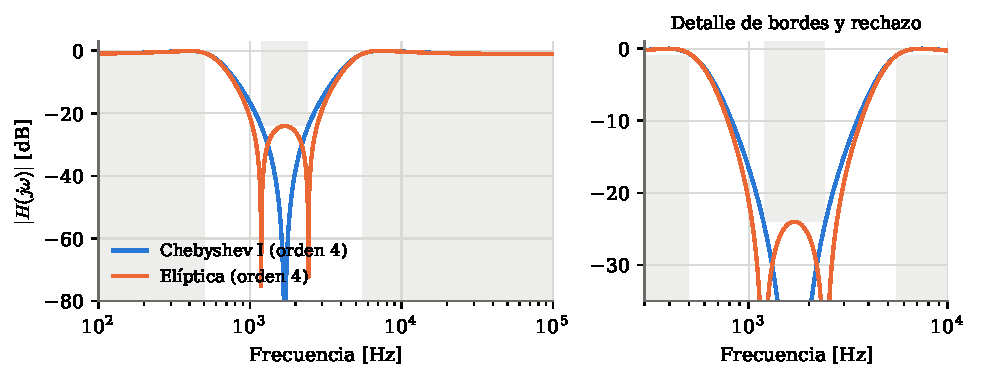
\includegraphics[width=\linewidth]{fig_BS_magnitud}
  \caption{Rechazabanda: magnitud de ambas aproximaciones y detalle de la transición.}
  \label{fig:BS_mag}
\end{figure}

En el LP (\cref{fig:LP_mag}) el elíptico resuelve la plantilla con orden~2 gracias al cero de transmisión en \qty{4005}{\hertz}, pero
su atenuación se estabiliza en \qty{24}{\decibel} por encima de esa frecuencia. El Chebyshev~I, en cambio, cae a
\qty{-60}{\decibel}/década sin límite: a \qty{10}{\kilo\hertz} atenúa \qty{66.1}{\decibel} frente a \qty{25.5}{\decibel} del
elíptico, una diferencia relevante para rechazar ruido y armónicos de alta frecuencia. En el BS (\cref{fig:BS_mag}), con el mismo orden,
el elíptico alcanza \qty{47.2}{\decibel} en los bordes de rechazo y empieza a atenuar \qty{24}{\decibel} desde \qty{1040}{\hertz}, frente a
\qty{1186}{\hertz} del Chebyshev~I, cuyo margen en los bordes es de solo \qty{0.62}{\decibel}.

\subsubsection{Fase y retardo de grupo}
El retardo de grupo se calcula analíticamente a partir de los polos $p_i = \sigma_{p_i}+j\omega_{p_i}$ y de los ceros
$z_j = \sigma_{z_j}+j\omega_{z_j}$ que no están sobre el eje $\jw$:
\begin{equation}
  \tau_g(\omega) = -\frac{d\varphi}{d\omega}
  = \sum_i \frac{-\sigma_{p_i}}{\sigma_{p_i}^2+(\omega-\omega_{p_i})^2}
  - \sum_j \frac{-\sigma_{z_j}}{\sigma_{z_j}^2+(\omega-\omega_{z_j})^2},
  \label{eq:retardo}
\end{equation}
y coincide con la derivada numérica de la fase desenrollada con error relativo menor que \num{4e-6}. Los ceros sobre $\jw$ solo
introducen saltos de fase de $\pm\ang{180}$ en $\omega_z$ (cambio de signo de $H$), visibles en las \cref{fig:fase,fig:fase_bs} para los elípticos.
En el BS Chebyshev~I el cero es doble, el salto es de \ang{360} y el desenrollado lo elimina.

\begin{figure}[H]
  \centering
  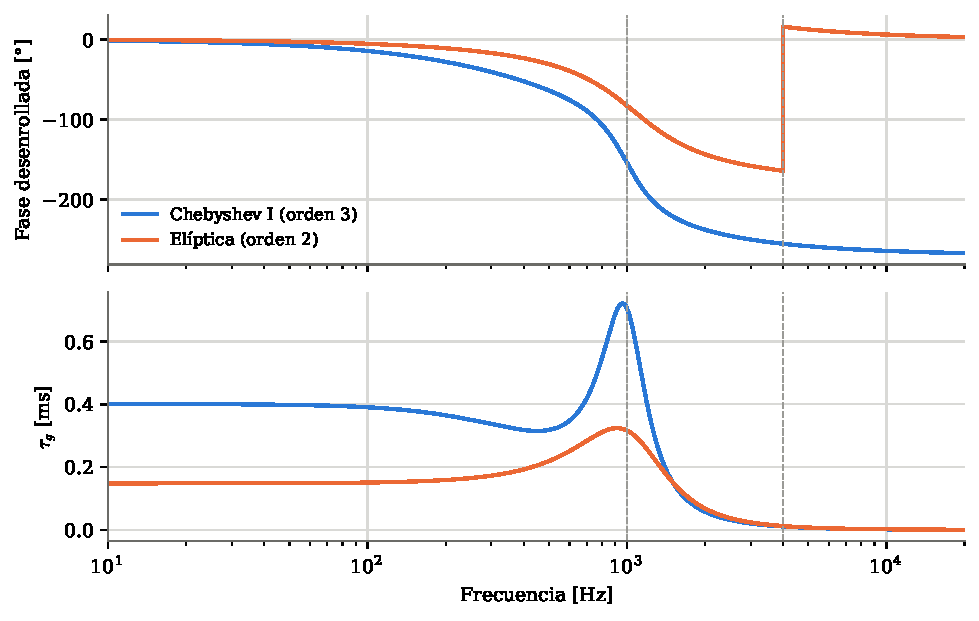
\includegraphics[width=0.92\linewidth]{fig_LP_fase_retardo}
  \caption{Pasabajos: fase desenrollada y retardo de grupo. Las líneas punteadas son los bordes de la plantilla.}
  \label{fig:fase}
\end{figure}

\begin{figure}[H]
  \centering
  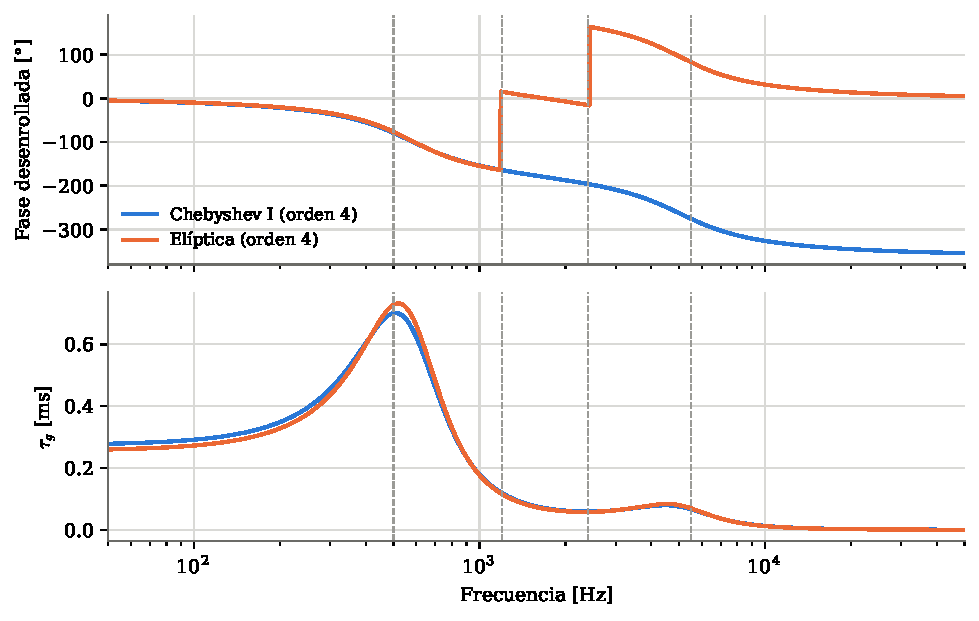
\includegraphics[width=0.92\linewidth]{fig_BS_fase_retardo}
  \caption{Rechazabanda: fase desenrollada y retardo de grupo. Los saltos de la fase del elíptico ocurren en sus ceros de transmisión.}
  \label{fig:fase_bs}
\end{figure}

\subsubsection{Respuesta temporal}

\begin{figure}[H]
  \centering
  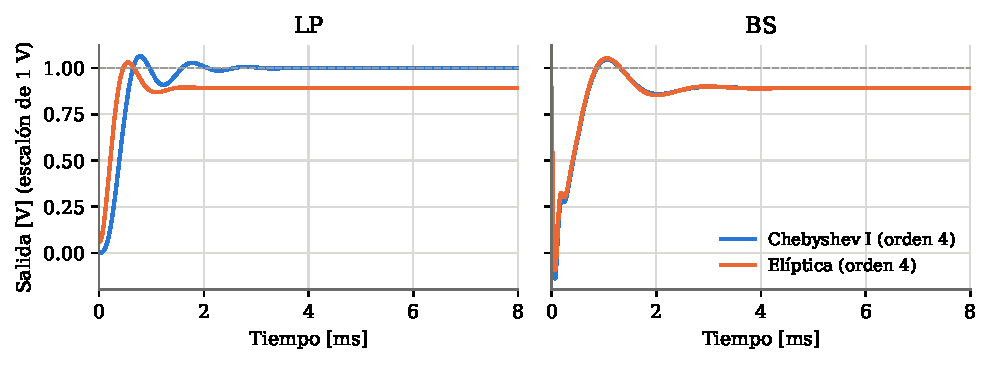
\includegraphics[width=\linewidth]{fig_escalon}
  \caption{Respuesta al escalón unitario.}
  \label{fig:escalon}
\end{figure}

\begin{table}[H]
  \centering\small
  \caption{Comparación de magnitud y de comportamiento temporal. $\Delta\tau_g$: variación del retardo de grupo en la banda de paso.}
  \label{tab:comparativa}
  \tabres{tab_comparativa_magnitud}\\[8pt]
  \tabres{tab_comparativa_tiempo}
\end{table}

La \cref{tab:comparativa} y la \cref{fig:escalon} muestran el compromiso típico entre selectividad y comportamiento temporal. El
Chebyshev~I de orden~3 tiene mayor retardo (\qty{0.40}{\milli\second} en continua) y un pico de \qty{0.72}{\milli\second} cerca del borde
de paso, con una variación de \qty{0.41}{\milli\second} dentro de la banda; su sobrepico es moderado (\qty{6.4}{\percent}) y se establece
al \qty{2}{\percent} en \qty{1.9}{\milli\second}. El elíptico de orden~2 tiene menos retardo pero más sobrepico (\qty{15.5}{\percent}) y,
como el grado de su numerador iguala al del denominador, su salida salta instantáneamente a $H(j\infty) = \num{0.063}$ ante el escalón.
En el BS ambas aproximaciones tienen retardo y respuesta al escalón casi idénticos, porque sus polos son muy parecidos (\cref{tab:secciones}).

\subsection{Elección del filtro y propuesta de implementación}
\label{sec:eleccion}

Se propone implementar el \textbf{pasabajos Chebyshev~I de orden~3} (propuesta de la cátedra, sujeta a aprobación docente). Los motivos
son los siguientes:
\begin{enumerate}
  \item \textbf{Margen de especificación.} Cumple con \qty{17.9}{\decibel} de margen en la banda de rechazo y sigue atenuando a
        \qty{-60}{\decibel}/década, lo que absorbe la dispersión de los componentes (relevante para el análisis de tolerancias del Nivel~II).
        Los elípticos tienen margen nulo por construcción.
  \item \textbf{Función todo polos.} Se realiza con una sección de primer orden y una bicuadrática pasabajos de un solo AO
        (Sallen--Key~\cite{daryanani1976}). Los demás casos requieren bicuadráticas con ceros sobre $\jw$ (secciones notch), con más AO y
        con alta sensibilidad de la frecuencia del cero.
  \item \textbf{Orden impar.} $H(0) = \qty{0}{\decibel}$, sin la pérdida de \qty{1}{\decibel} en continua de los diseños de orden par.
  \item \textbf{$Q$ moderado.} $Q = \num{2.018}$ es realizable con AO de propósito general; la verificación de GBW y slew rate se hace en
        la etapa de selección del AO.
\end{enumerate}
Su contracara es el mayor retardo de grupo y su variación cerca del borde de paso, que es precisamente lo que motiva el ecualizador de
fase del Nivel~III.

\paragraph{Orden de la cascada.} La bicuadrática aislada presenta un pico de $Q/\sqrt{1-1/(4Q^2)} \to \qty{6.37}{\decibel}$ en
\qty{934}{\hertz} (\cref{fig:secciones}). Si se ubicara primero, la señal en el nodo intermedio superaría en \qty{6.4}{\decibel} a la de la
salida y limitaría la amplitud máxima de entrada antes de saturar. Ubicando primero la sección de primer orden, el nodo intermedio nunca
supera la ganancia unitaria, de modo que la salida final es el punto de mayor nivel.

\begin{figure}[H]
  \centering
  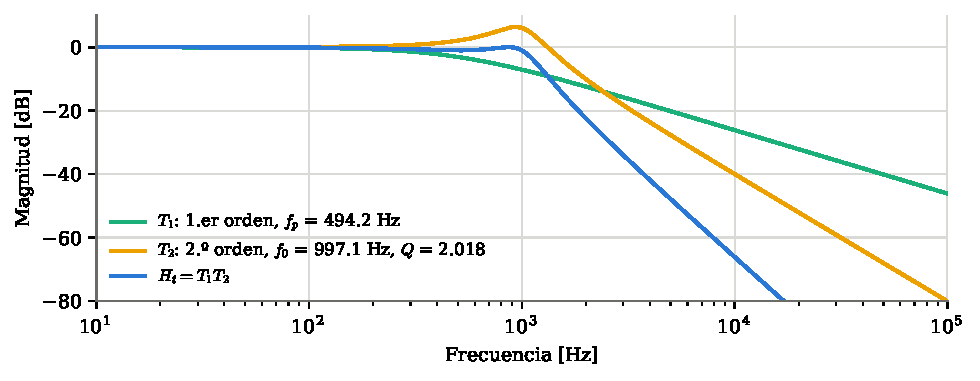
\includegraphics[width=0.85\linewidth]{fig_LP_cheby1_secciones}
  \caption{Descomposición del LP Chebyshev~I en $T_1(s)$ (primer orden) y $T_2(s)$ (bicuadrática). El producto reproduce $H_t(s)$ con
  error menor que \num{1e-15}.}
  \label{fig:secciones}
\end{figure}

\paragraph{Propuesta de implementación.} Etapa~1: polo real con una red RC seguida de un seguidor de tensión, que aísla la red y entrega
a la etapa siguiente la baja impedancia de fuente que exige el Sallen--Key. Etapa~2: Sallen--Key pasabajos para el par complejo. Ambos AO en un
TL072. La síntesis (\cref{sec:sintesis}) incorpora además un \emph{margen de diseño}: como $H_t$ tiene exactamente \qty{1}{\decibel} de rizado,
se sintetiza una función Chebyshev~I de orden~3 algo más exigente, para que las tolerancias de los componentes no lleven el filtro construido fuera
de la plantilla.
